\section{Arbeitsintegrale}
\subsection{Arbeit als Skalarprodukt}
Physikalische Grössen mit einer Richtung wie Kraft oder Geschwindigkeit werden mit Vektoren beschrieben. Bei anderen Grössen wie Temperatur, Masse oder Arbeit handelt es sich jedoch um sogenannte Skalare grössen - also um solche, die mit einer Zahl beschrieben werden. Die Verbindung zwischen vektoriellen und skalaren Grössen geschieht häufig mit dem Skalarprodukt von Vektoren.

\begin{bsp}
    {Arbeit als Skalarprodukt}{intro-Arbeit}
    Wenn unter Wirkung einer Kraft einen Weg zurückgelegt wird, wird mechanische Arbeit verrichtet. Betrachten Sie beispielsweise einen Wagen, der sich auf einer Schiene befindet und auf den seitwärts eine konstante Kraft $F$ wirkt

    \begin{center}
        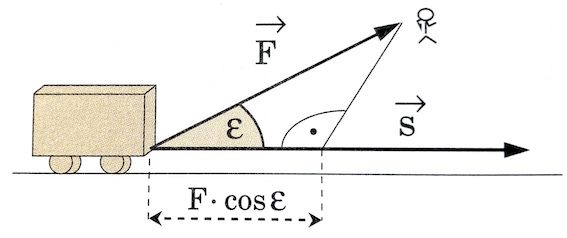
\includegraphics[width = 0.5\textwidth]{skalarprodArbeit.jpg}
    \end{center}

    

    Die Arbeit $W$ ist in diesem Fall das Produkt aus dem zurückgelegten Weg $s$ und der \emph{Komponente der Kraft längs der Schiene}:
    $$ W = \lvert\vec{F}\rvert  \cdot \cos(\varepsilon) \cdot s$$

    Die Kraftkomponente, die parallel zur Schiene verläuft, wird häufig mit dem Skalarprodukt berechnet. Wir erinnern uns an die Definition des Skalarprodukts:
    $$\langle \vec{a} , \vec{b} \rangle = \lvert\vec{a}\rvert\cdot \lvert\vec{b}\rvert \cdot \cos(\varepsilon)$$
    Somit gilt
    $$ \lvert\vec{F}\rvert  \cdot \cos(\varepsilon) = \left\langle\vec{F},  \vec{s}\right \rangle \cdot \frac{1}{\lvert\vec{s}\rvert} = \left\langle \vec{F} , \frac{\vec{s}}{\lvert\vec{s}\rvert} \right \rangle$$
    Die mechanische Arbeit, die bei der Bewegung des Wagens auf der Schiene verrichtet wird, kann schliesslich so berechnet werden:
    $$W = \left\langle\vec{F} , \frac{\vec{s}}{\lvert\vec{s}\rvert}\right\rangle \cdot s $$
    Das scheint auf den ersten Blick komplizierter als die erste Formel zu sein, diese Darstellung lässt sich jedoch gut auf die Situation übertragen, wenn die Bewegung entlang einer Kurve geschieht.

\end{bsp}

\clearpage

% In der letzten Formel im \Cref*{bsp:intro-Arbeit} oben, haben die beiden darin vorkommenden ``$\cdot$''-Zeichen zwei unterschiedliche Bedeutungen. Das erste $\cdot$ innerhalb der Klammern steht für das Skalarprodukt von zwei Vektoren. Das zweite hingegen für die Multiplikation von zwei reellen Zahlen. Damit es nicht zu Verwechslungen kommt – insbesondere auch darum, weil wir teilweise auf die Vektorpfeile verzichten – führen wir für das Skalarprodukt die Notation ein, die auch an Hochschulen verwendet wird: 

% \begin{definition}
%     {Schreibweise für das Skalarprodukt}{}
%     Seien $\vec{a}$ und $\vec{b}$ zwei Vektoren. Dann schreiben wir für das Skalarprodukt der beiden Vektoren
%     $$\langle \vec{a}, \vec{b} \rangle $$

% \end{definition}

% Mit dieser Schreibweise lautet die Formel für die mechanische Arbeit aus  \Cref*{bsp:intro-Arbeit}:
% $$W = \langle \vec{F}, \frac{\vec{s}}{\lvert\vec{s}\rvert}\rangle \cdot s $$


\subsection{Arbeit entlang eines Weges in einem Kraftfeld}
Im Folgenden soll die Situation mit dem Wagen aus \Cref*{bsp:intro-Arbeit} auf zwei Arten verallgemeinert werden: Die wirkende Kraft $\vec{F}$  soll nicht mehr konstant sein und die Bewegung soll nicht mehr entlang einer Geraden stattfinden.

\emph{Aus der Kraft wird ein Kraftfeld}

Beginnen wir damit, dass die Kraft nicht mehr konstant ist. Damit ist gemeint, dass die wirkende Kraft abhängig ist vom Ort, an dem sich das Objekt befinden. In anderen Worten: Jedem Ort in wird eine Kraft zugeordnet. Das ist eine Funktion!
\begin{definition}
    {Vektorfelder}{vektorfeld}
    Ein Vektorfeld ist eine Funktion, die jedem Punkt in der Ebene (oder im Raum) einen Vektor zuordnet.

    Ein Vektorfeld ist somit eine Abbildung der Form:
    $$ \vec{V} : \R^2 \to \R^2$$
\end{definition}
Vektorfelder stellt man sich am besten so vor: Jedem Punkt der Ebene wird ein Vektor zugeordnet, der von diesem Punkt aus startet.

\begin{center}
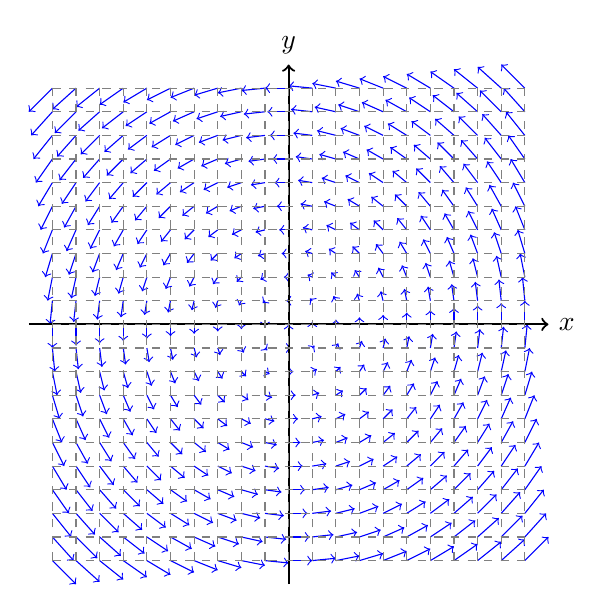
\begin{tikzpicture}[scale = 0.3]
    \foreach \x in {-10,-9,...,10}
        \foreach \y in {-10,-9,...,10}
            \draw[->, blue] (\x,\y) -- (\x-\y/10,\y+\x/10);

    % Achsen
    \draw[thick,->] (-11,0) -- (11,0) node[right] {$x$};
    \draw[thick,->] (0,-11) -- (0,11) node[above] {$y$};
    
    % Gitterlinien
    \foreach \x in {-10,-9,...,10}
        \draw[thin, gray, dashed] (\x,-10) -- (\x,10);
    \foreach \y in {-10,-9,...,10}
        \draw[thin, gray, dashed] (-10,\y) -- (10,\y);
\end{tikzpicture}
\end{center}

Die physikalische Bedeutung solcher Vektorfelder kann ganz unterschiedlich sein. Wir werden Sie häufig als Kraftfelder betrachten. Der Bildvektor ist dann die an der betrachteten Position wirkende Kraft. Mit Vektorfelder kann aber zum Beispiel auch die Strömung einer Flüssigkeit beschrieben werden. In diesem Fall steht der Bildvektor für die Geschwindigkeit der Flüssigkeit an der betrachteten Stelle.

\clearpage

\emph{Aus der geraden Schiene wird eine Kurve}

Wir kommen nun zur zweiten Verallgemeinerung des \Cref*{bsp:intro-Arbeit}. Anders als im Beispiel soll die Bewegung entlang einer Kurve stattfinden, von der die Parametrisierung gegeben ist: $$\vec{r}: [a,b]\to\R^2,\quad  t\mapsto \vec{r}(t)$$

\begin{center}
    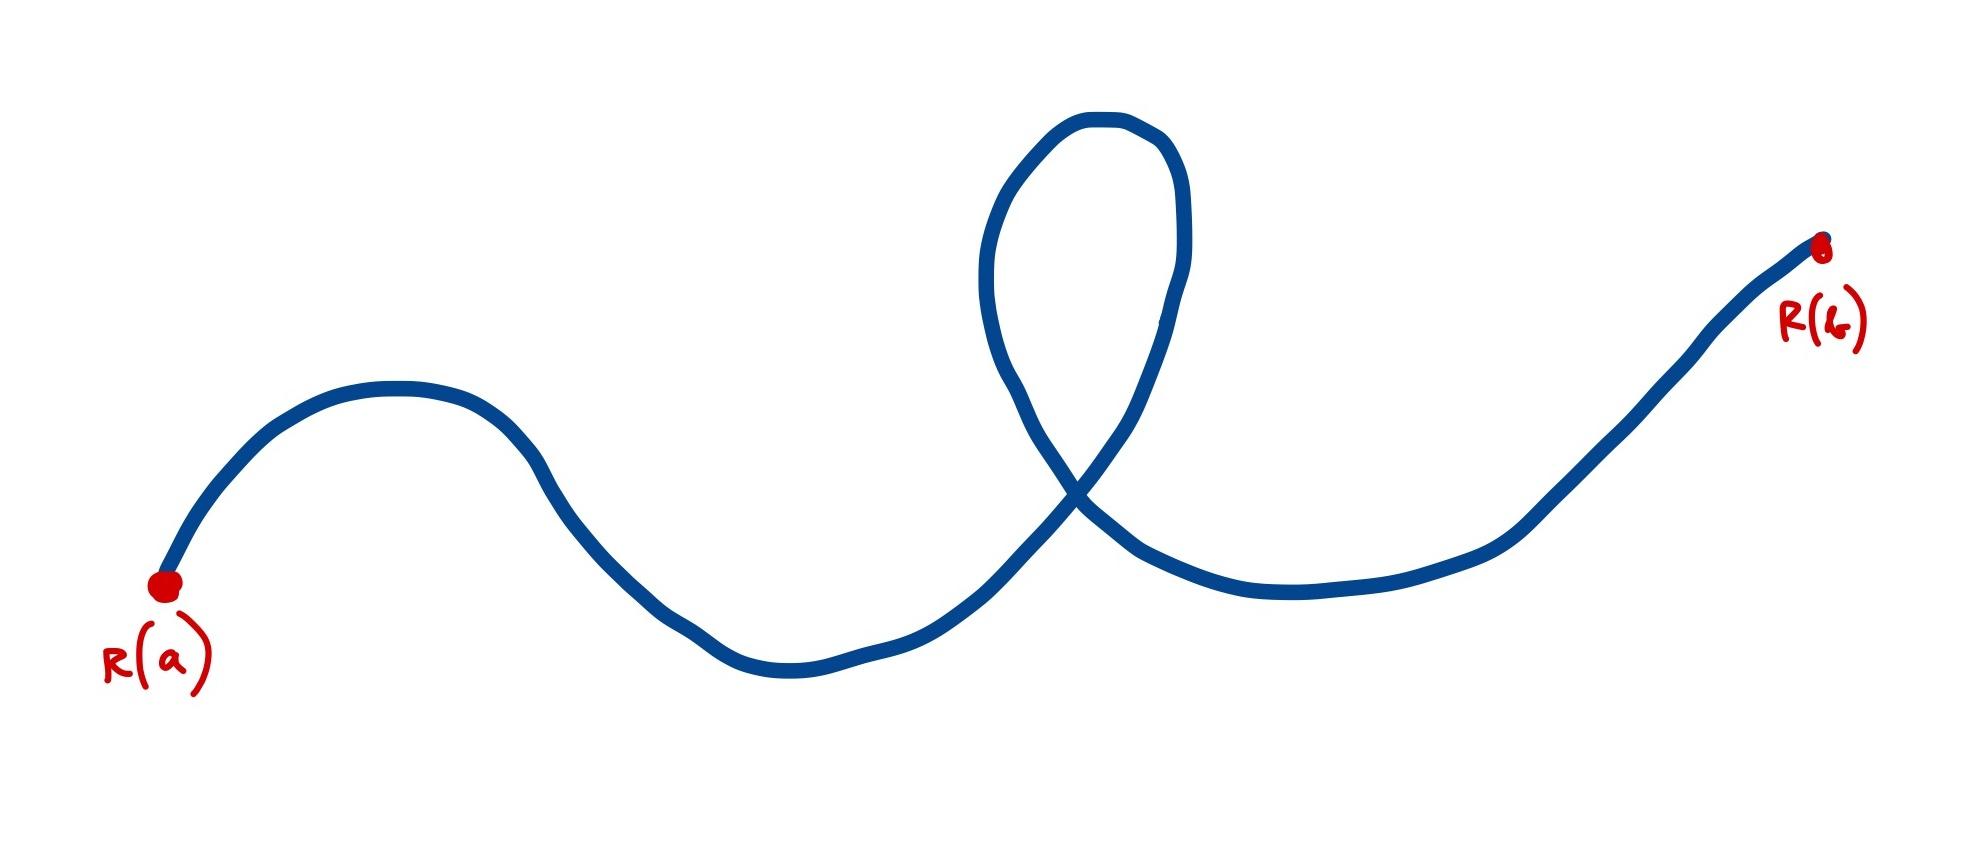
\includegraphics[width = 0.7\textwidth]{ArbeitsintegralSkizze1.jpg}
\end{center}

Um die verrichtete Arbeit näherungsweise zu bestimmen, wird das Intervall $[a,b]$ in $n$ kleine Teilintervalle mit den Grenzen $a=t_0, t_1, t_2, \dots, t_n = b$ unterteilt. Die entsprechenden Kurvenstücke sind dann nahezu gerade. Damit kann die Arbeit für ein solches Kurvenstück mit der Formel $W = \left\langle \vec{F}, \frac{\vec{s}}{\lvert\vec{s}\rvert}\right\rangle \cdot s$ für die Arbeit entlang einer Geraden approximiert werden.  Für die verrichtete Arbeit $W_k$ im Zeitintervall $[t_k, t_{k+1}]$ gilt: 
$$W_k \approx \left\langle \vec{F}(\vec{r}(t_k)), \frac{\dot{\vec{r}}(t_k)}{\lvert\dot{\vec{r}}(t_k)\rvert} \right\rangle \cdot \Delta s$$

\begin{center}
    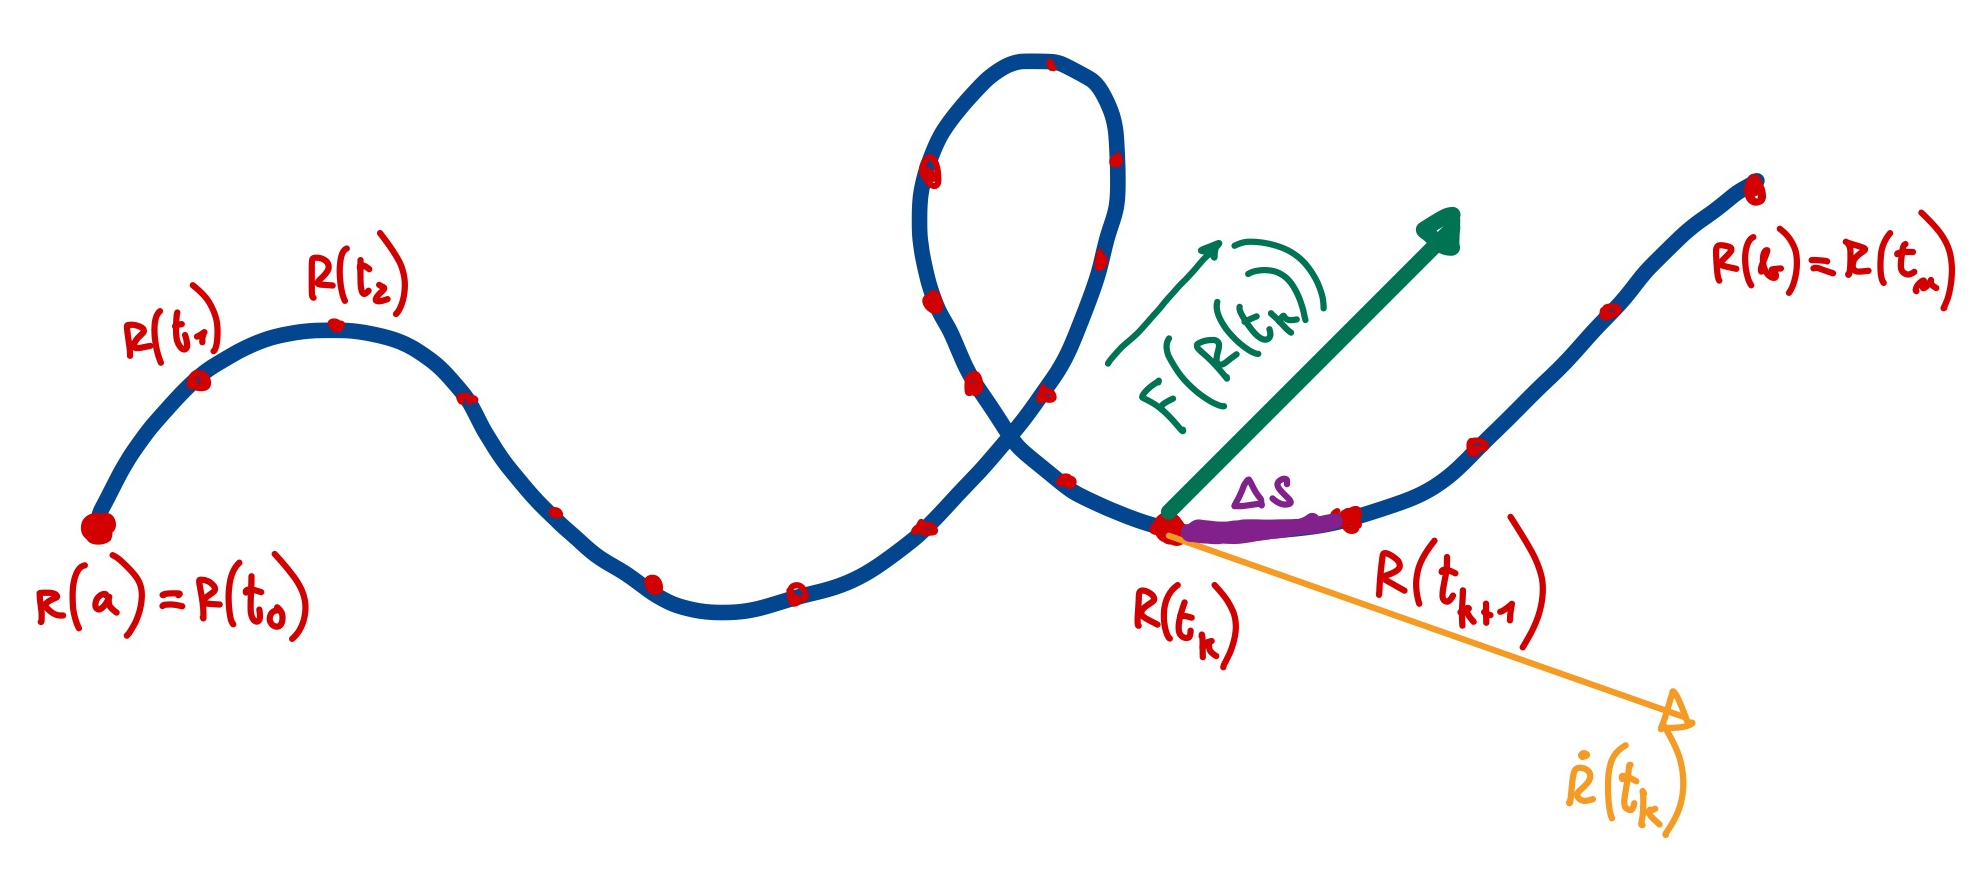
\includegraphics[width = 0.7\textwidth]{ArbeitsintegralSkizze2V2.png}
\end{center}

Diese Formel kann etwas vereinfacht werden, wenn man berücksichtigt, dass der im Intervall $[t_k, t_{k+1}]$ zurückgelegte Weg $\Delta s$ aus der Schnelligkeit $|\dot{\vec{r}}(t_k)|$ und der verstrichenen Zeit $\Delta t = t_{k+1} - t_k$ berechnet werden kann: $\Delta s = |\dot{\vec{r}}(t_k)|\cdot \Delta t$. Somit folgt:

$$W_k \approx \left\langle \vec{F}(\vec{r}(t_k)), \frac{\dot{\vec{r}}(t_k)}{\lvert\dot{\vec{r}}(t_k)\rvert} \right\rangle \cdot |\dot{\vec{r}}(t_k)|\cdot \Delta t = \left\langle \vec{F}(\vec{r}(t_k)), \dot{\vec{r}}(t_k) \right\rangle \cdot \Delta t $$


Für die gesamte Arbeit gilt dann:
$$W \approx \sum_{k=0}^{n} \left\langle \vec{F}(\vec{r}(t_k)), \dot{\vec{r}}(t_k) \right\rangle \cdot \Delta t$$
Diese Approximation wird umso besser, je mehr und je kleiner die Teilintervalle sind. Für $n\to\infty$ erhält man schliesslich:
$$ W = \int_{a}^{b} \left\langle \vec{F}(\vec{r}(t)), \dot{\vec{r}}(t) \right\rangle  \,  dt$$

\begin{definition}
    {Arbeitsintegrale}{Arbeitsintegral oder Wegintegrale 2. Art}
    Sei $\vec{F}: \R^2\to\R^2$ ein Vektorfeld und $\vec{r}: [a,b]\to\R^2, \, t\mapsto \vec{r}(t)$ eine parametrisierte Kurve. Dann ist das Arbeitsintegral von $\vec{F}$ entlang der Kurve $\vec{r}$ definiert als
    $$ W = \int_{a}^{b} \left\langle \vec{F}\left(\vec{r}(t)\right), \dot{\vec{r}}(t) \right\rangle  \,  dt$$
    Man schreibt dafür kurz
    $$W =\int_{\vec{r}} \vec{F} \, d\vec{s}$$
\end{definition}

\begin{bsp}{Arbeitsintegral im Wirbelfeld}{Wirbelfeld2Wege}
    Gegeben ist das Vektorfeld $\vec{F}(x,y) = \begin{pmatrix}
        -y \\x
    \end{pmatrix}$ und die Kurven $\vec{r}_1 : [0,1]\to \R^2, \,  t \mapsto \begin{pmatrix}
        1-2t \\ 0
    \end{pmatrix}  $ und $\vec{r}_2 : [0, \pi]\to \R^2, \,  t \mapsto \begin{pmatrix}
        \cos t \\ \sin t
    \end{pmatrix}  $
    
    Gesucht sind die beiden Arbeitsintegrale  $\int_{\vec{r}_1} \vec{F} \, d\vec{s}$ und $\int_{\vec{r}_2} \vec{F} \, d\vec{s}$
    \vspace*{5cm}

    \pagebreak
    \phantom{2}

    \vspace*{12cm}
\end{bsp}


\begin{ueb}
    {}{}
    Ein Kraftfeld $\vec{F}:\mathbb{R}^3\longrightarrow \mathbb{R}^3$ sei durch
$$\vec{F} : \, (x,y,z) \; \longmapsto \; 
\left( \begin{array}{c}
x \\
yz \\
z^2-x
\end{array}\right) $$
gegeben. 


Berechnen Sie die Arbeit, die verrichtet wird, wenn ein Massenpunkt entlang der parametrisierten Wege $\vec{c}_1$ bzw. $\vec{c}_2$ verschoben wird, wobei die beiden Kurven $\vec{c}_{1,2}:[0,1]\longrightarrow \mathbb{R}^3$, gegeben sind durch
$$\vec{c}_1(t) \; = \; \left( \begin{array}{c}
t \\
1-t \\
t
\end{array}\right) 
\hspace{1cm} \mbox{bzw.} \hspace{1cm}
\vec{c}_2(t) \; = \; \left( \begin{array}{c}
t^2 \\
1-t \\
t
\end{array}\right) $$
und beide die Punkte $A=(0,1,0)$ und $B=(1,0,1)$ miteinander verbinden.
\end{ueb}

\emph{Lösung:} $W_1 = \frac{1}{6}, \quad W_2 = \frac{1}{3}$









